\section{Open Data}

\frame{
\frametitle{Open Data}
\begin{definiere} [OpenData]
"Open Data ist eine Philosophie und Praxis, die zur Grundlage hat, dass Daten frei f�r jedermann verf�gbar und frei von Copyrights, Patenten oder anderen Kontrollmechanismen sind." - Wikipedia
\end{definiere}}

\frame{
\frametitle{Open Data}
\begin{kasten} [Rechtsgrundlage]
Das "Informationsfreiheitsgesetz vom 5. September 2005 (BGBl. I S. 2722)" bildet einen juristischen Pfeiler f�r die Handhabe "offener Daten": \baselineskip \baselineskip

"� 1 Grundsatz (1) Jeder hat nach Ma�gabe dieses Gesetzes gegen�ber den Beh�rden des Bundes einen Anspruch auf Zugang zu amtlichen Informationen."\baselineskip \baselineskip

"� 2 Begriffsbestimmungen. Im Sinne dieses Gesetzes ist amtliche Information: jede amtlichen Zwecken dienende Aufzeichnung, unabh�ngig von der Art ihrer Speicherung [...]."
\end{kasten}}

\frame{
\frametitle{OpenData Network}
\begin{kasten}[OpenData Network]
Das OpenData Network propagiert die nutzbringende Verwendung offener Daten. \baselineskip \baselineskip

Grunds�tze des OpenData Networks:
	\begin{itemize}
	   \item Informationsfreiheit
	   \item B�rgerrechte in der Informationsgesellschaft
	   \item Kollaborative Formen der Partizipation
	\end{itemize}
\end{kasten}}

\frame{
\frametitle{OpenData Network}
\begin{merkmale} [OpenData Principles]
	\begin{itemize}
 	   \item Vollst�ndigkeit
 	   \item Prim�rquelle
 	   \item Zeitnah
 	   \item Zug�nglichkeit
	   \item Maschinenlesbar
	   \item Nicht diskriminierend
 	   \item Nicht propri�ter
 	   \item Lizenzfrei
	\end{itemize}
\end{merkmale}}

\frame{
\frametitle{Geodaten}
\begin{kasten}[Inspire Richtlinie 2004/0175]
Ziel der EU-Inspire Richtlinie 2004/0175\baselineskip
"Schaffung einer Geodateninfrastruktur in der Europ�ischen Gemeinschaft"
\end{kasten}}

\frame{
\frametitle{Geodaten}
\begin{merkmale}[Geodaten]
\begin{itemize}
  \item Bessere Handlungsm�glichkeiten bei der Bek�mpfung von Umweltproblemen
  \item Verwendung von Wetterbildern und Verkehrsstr�men
\end{itemize}
\end{merkmale}}

\frame{
\frametitle{Beispiel: Offener Haushalt}
\begin{merkmale}[Offener Haushalt]
\begin{itemize}
  \item Verwendung der Daten des Finanzministeriums
  \item Visuelle Aufbereitung der Daten ohne Verlust von Details
  \item M�glichkeit der Weiterverarbeitung der Daten
\end{itemize}
\end{merkmale}
}

\frame{
\frametitle{Beispiel: Offener Haushalt}
\begin{figure}
\begin{center}
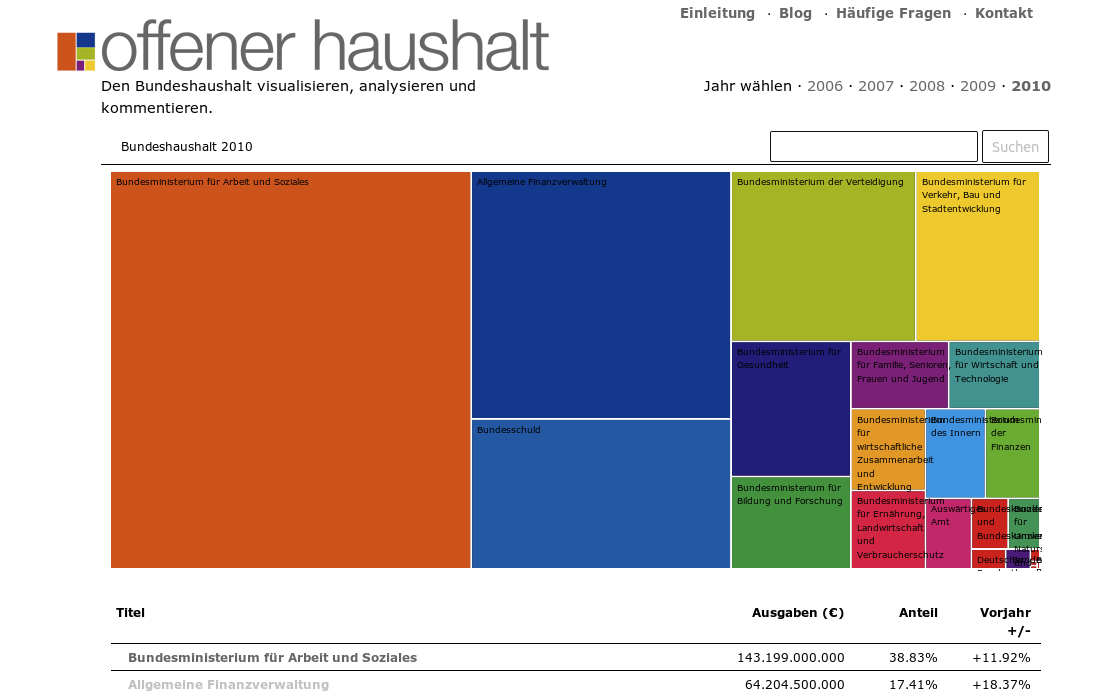
\includegraphics[width=10cm]{./images/Screen_offener_Haushalt.png}
\caption{Screenshot der Seite bund.offenerhaushalt.de, November 2010}
\end{center}
\end{figure}
}

\frame{
\frametitle{Beispiel: B�rgerhaushalt K�ln}
\begin{merkmale}[B�rgerhaushalt K�ln]
\begin{itemize}
  \item Abgabe, Bewertung und Diskussion von/�ber Vorschl�ge
  \item Anschlie�ende Pr�fung der jeweils besten 100 Vorschl�ge der Bereiche "Schule / Bildung" und "Umweltschutz" 
  \item Abschlie�end begr�ndete Entscheidung �ber die Vorschl�ge durch den Rat der Stadt K�ln
\end{itemize}
\end{merkmale}}

\frame{
\frametitle{Beispiel:B�rgerhaushalt K�ln}
\begin{figure}
\begin{center}
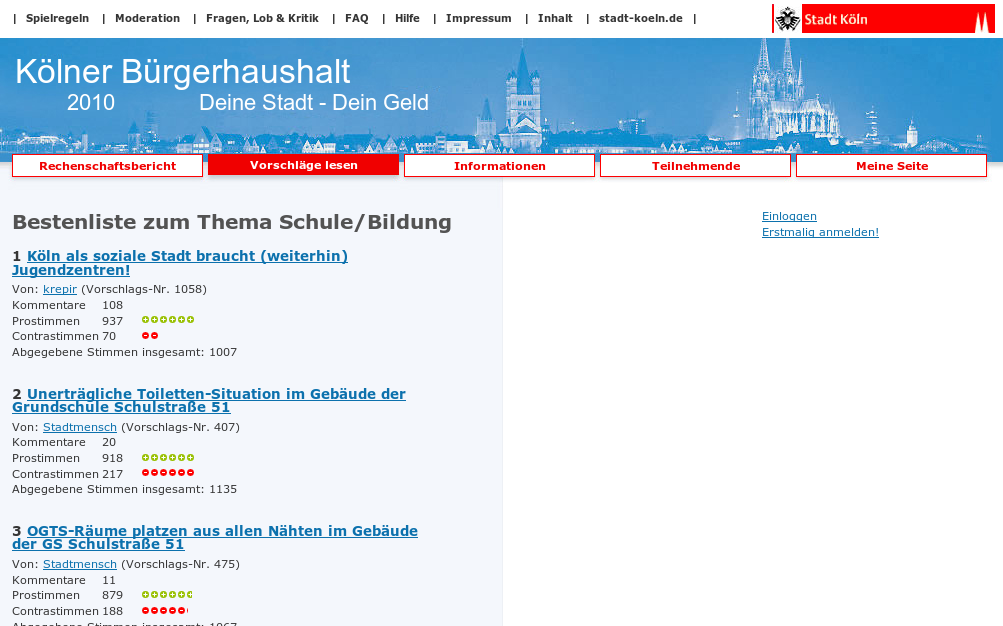
\includegraphics[width=10cm]{./images/Screen_Buergerhaushalt.png}
\caption{Ausschnitt der Seite buergerhaushalt.stadt-koeln.de, November 2010}
\end{center}
\end{figure}}

\frame{
\frametitle{Beispiel: Fix My Street}
\begin{kasten}[ Funktionsweise von Fix My Street]
\begin{itemize}
  \item Melden und Diskutieren von �rtlichen Problemen (z.B. Vandalismus, Defekte)
  \item Weiterleitung an die Zust�ndige �ffentliche Stelle
  \item R�ckmeldung �ber beschlossenen Ma�nahmen auf Fix My Street durch B�rgerInnen
\end{itemize}
\end{merkmale}}

\frame{
\frametitle{Beispiel: Fix My Street}
\begin{figure}
\begin{center}
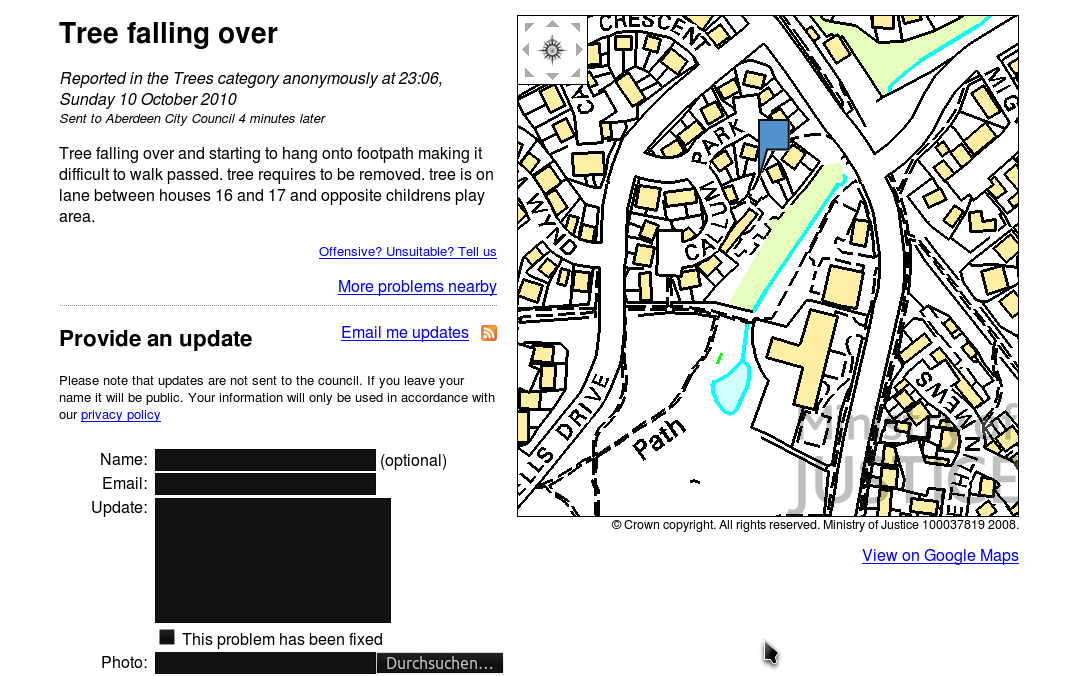
\includegraphics[width=10cm]{./images/Screen_Fixmystreet.png}
\caption{Ausschnitt der Seite www.fixmystreet.de, November 2010}
\end{center}
\end{figure}}

\frame{
\frametitle{Besipiel: Hackday}
\begin{definiere} [Hackday]
Hackdays sind Treffen, die das Ziel haben, zu zeigen, dass ohne gro�es Budget und in einem knappen Zeitrahmen n�tzliche Anwendungen programmiert werden k�nnen, mit denen die �ffentlichen Daten nutzbar werden.
\end{definiere}}
